\documentclass[../report.tex]{subfiles}
\begin{document}
\section{Website}
\subsection{Login Screen: index.html}
\begin{figure}[H]
	\centering
	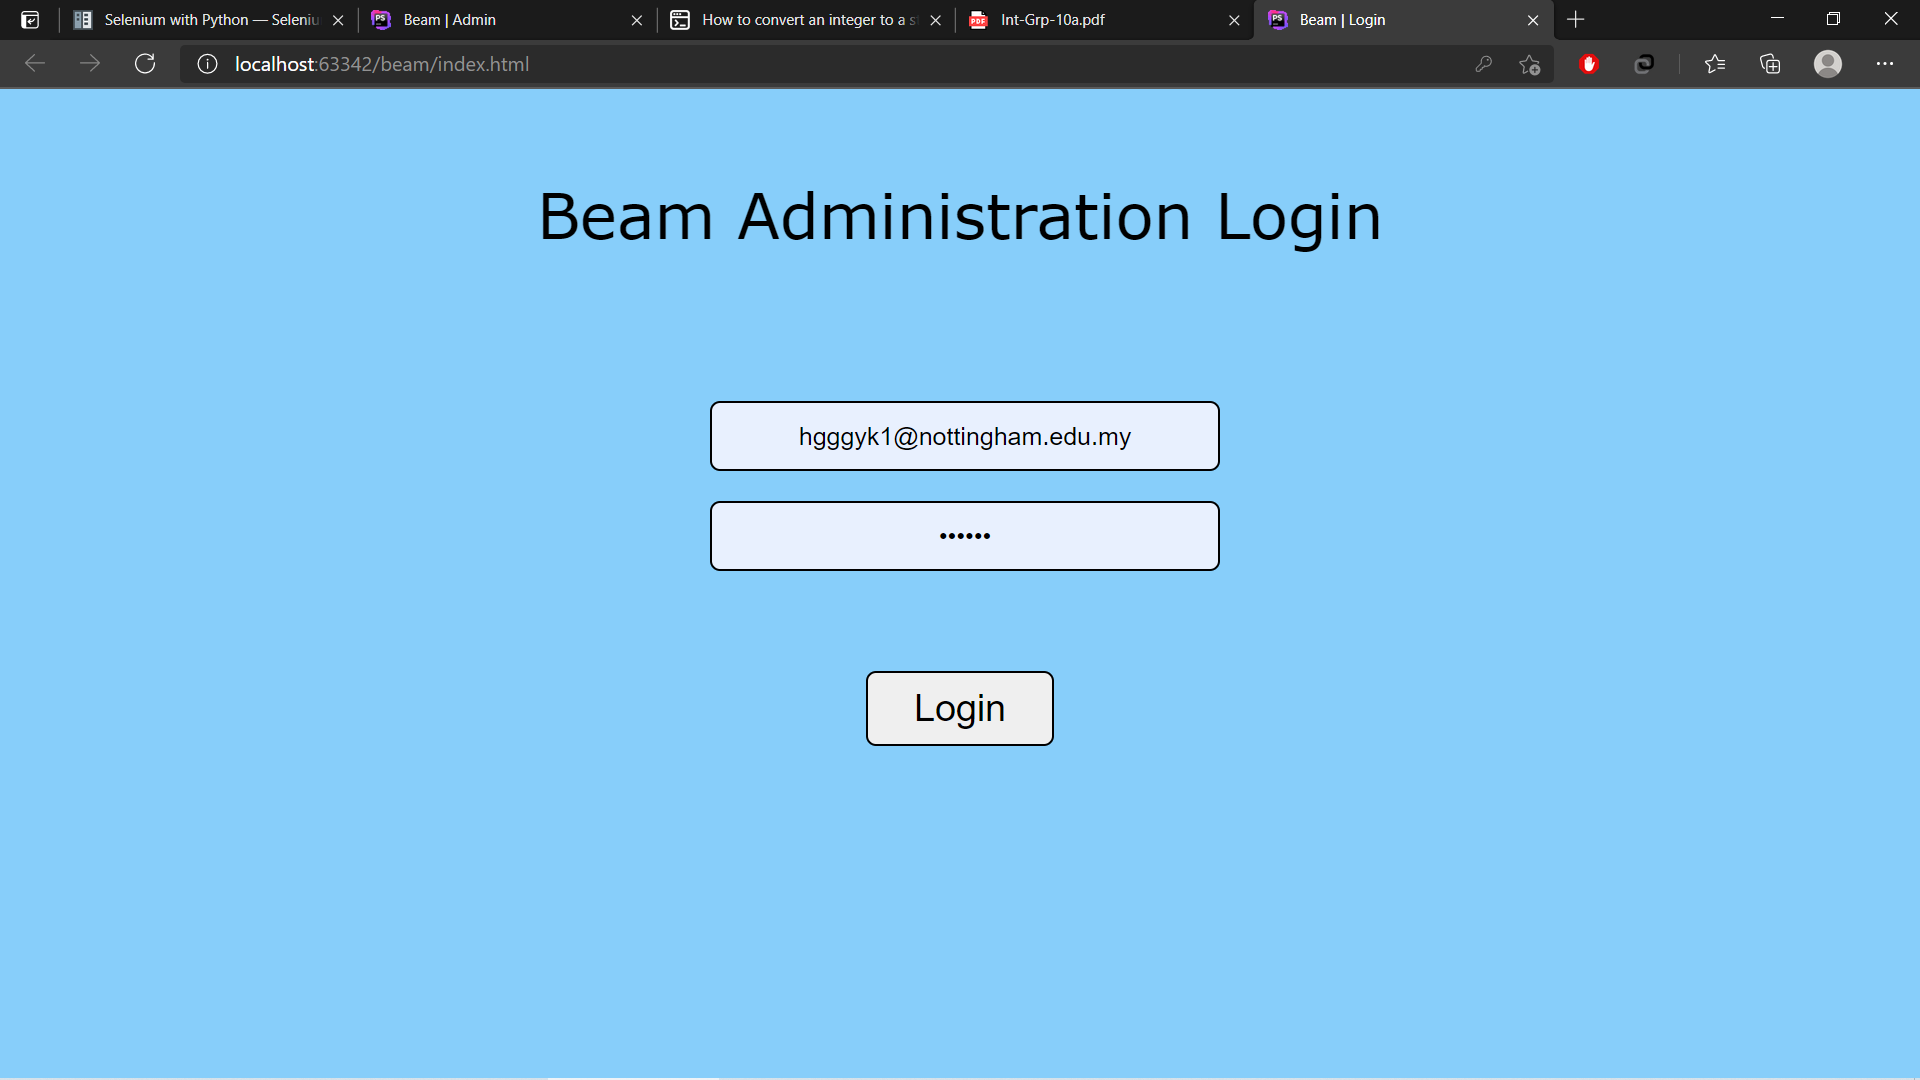
\includegraphics[width=.7\linewidth]{../images/07/01-01-login.png}
	\caption{Login interface of the website}
	\label{fig:07-01-01-login}
\end{figure}

The login interface comprises of a title -- Beam Administration Login, an input field for email, and an input field for password. Upon clicking to the login button, the \textit{login()} function will be executed, as shown below.

\lstinputlisting[language=JavaScript,firstline=36,lastline=50]{../code/web-index.html}

The \textit{login} function takes the email and password entered by the user and sends a promise to Firebase Authentication to check the login credentials. If the credentials are valid, the authentication state will be changed because of a successful user account login and the user will be redirected to \textit{home.html}. The user will remain logged in unless the account is logged out or the user switched to a new tab or window. The state of being logged in will only persist in the current tab or session, and it will be cleared of the tab or window is closed. 

\lstinputlisting[language=JavaScript,firstline=367,lastline=378]{../code/web-home.html}

The \textit{logOut} function logs the user out from the account and redirects the user back to the login page. If the user accesses the home page without going through the login page, the system will check if the user has logged in on Firebase Authentication. If not, the user will be redirected to the login page. The user will remain on the home page if Firebase Authentication detects that the user has performed a successful login.

\subsection{Home Screen: home.html}
\subsubsection{Home Component}
\begin{figure}[H]
	\centering
	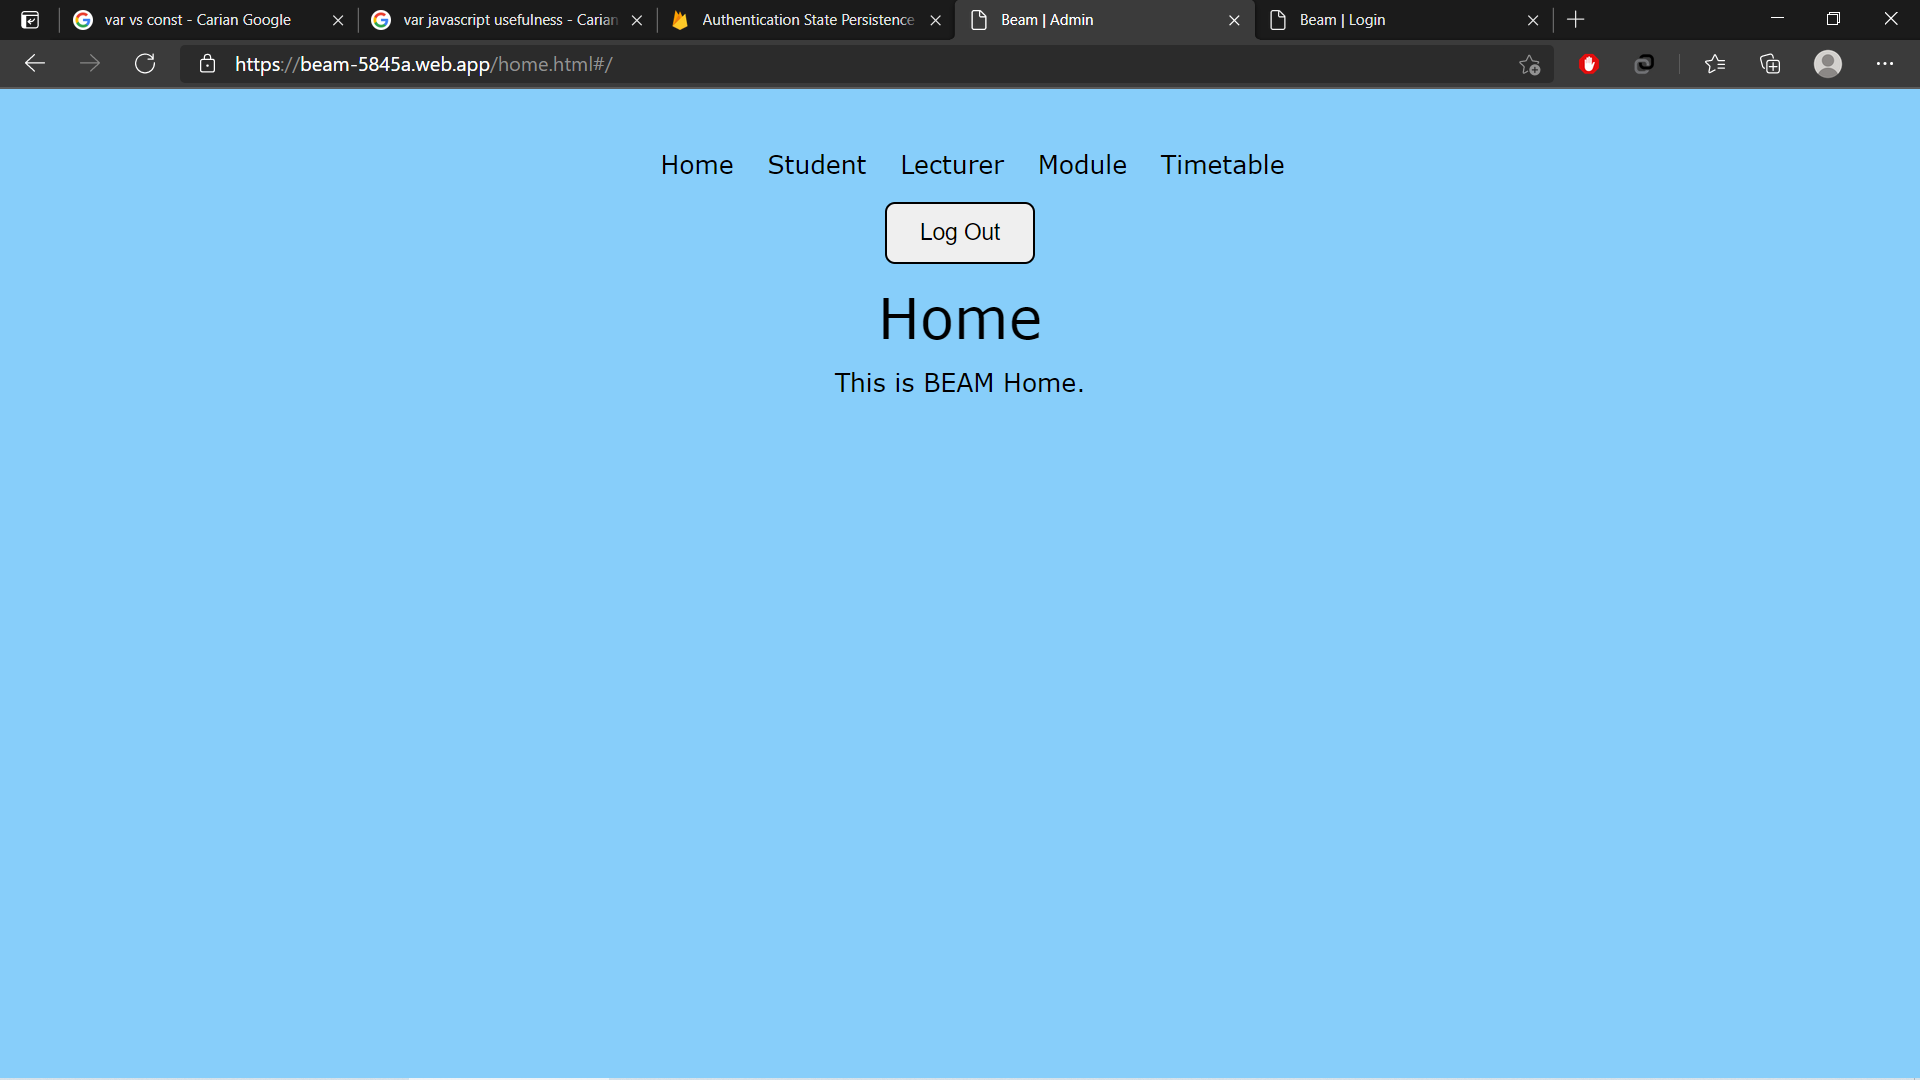
\includegraphics[width=.7\linewidth]{../images/07/01-02-home.png}
	\caption{This is the Home interface of the website. Note that it changed to any important announcement from the university}
	\label{fig:07-01-02-home}
\end{figure}

\lstinputlisting[language=JavaScript,firstline=86,lastline=105]{../code/web-home.html}

This home page is a \textit{single-page application (SPA)} that contains all the features needed for the admin to enter data into the database. Vue.js functions are imported using CDN and used to enable us to build a \textit{SPA}. This Vue.js \textit{SPA} is created in a \textit{$<$div$>$} with an id of \textit{app} with a \textit{router} to link each tab of the navigation with a path. The router will load the contents of each tab in \textit{hash} mode, which means \# is used before the navigation path is passed internally. Since this section of the URL is not sent to the server, no special treatment is required on the server level.
 
The code above directs each path to a component. Every component is an x-template, where the html elements (front-end) of a template in stored in a \textit{$<$script$>$} tag in a HTML file. The router will redirect the tabs to their respective template.

\bigskip
\subsubsection{Student Component}
\begin{figure}[H]
	\centering
	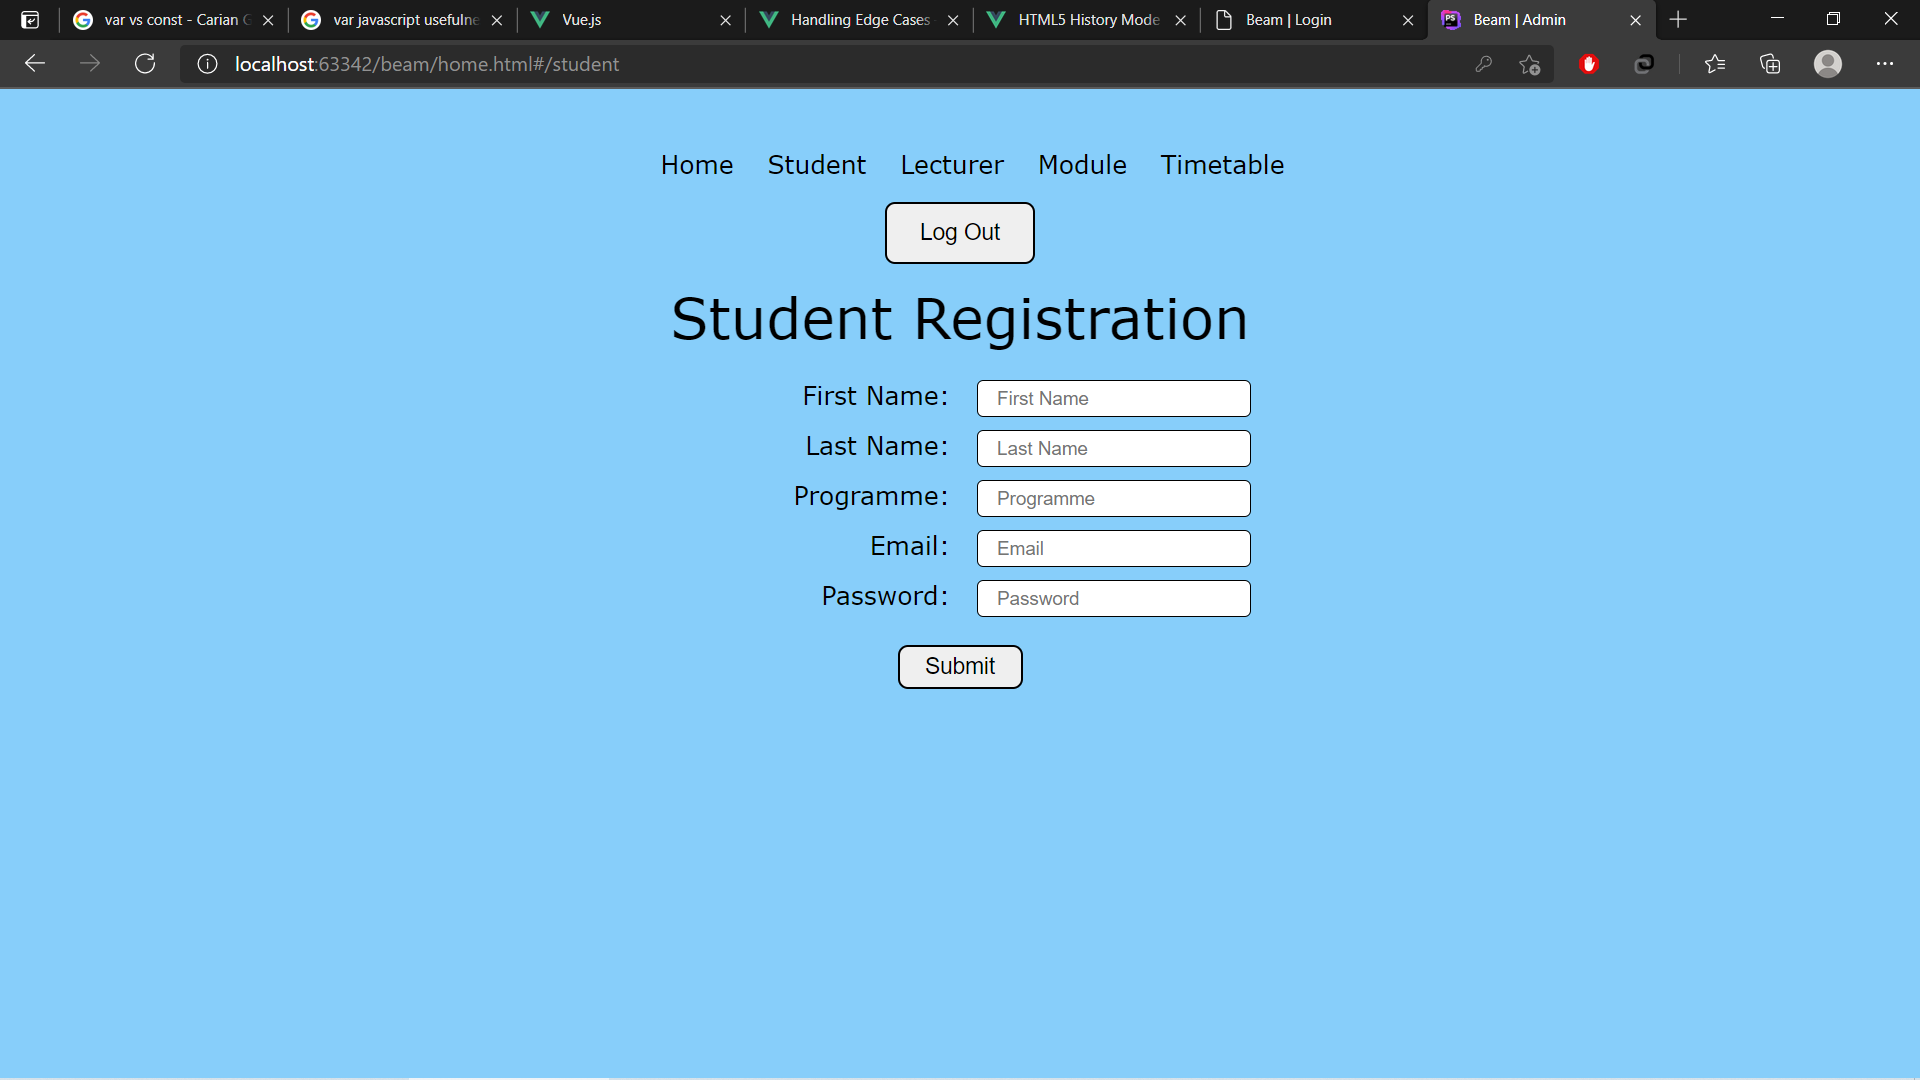
\includegraphics[width=.7\linewidth]{../images/07/01-03-student-reg.png}
	\caption{This is the Student Registration interface of the website}
	\label{fig:07-01-03-student}
\end{figure}

\lstinputlisting[language=JavaScript,firstline=144,lastline=166]{../code/web-home.html}

When the \textit{email} and \textit{password} are sent to Firebase Authentication to create a new account for the student, the \textit{first name}, \textit{last name}, \textit{programme}, and \textit{email}, are entered under the \textit{student} node and grouped by the student account’s \textit{user uid}. Under the \textit{users} node, the role of the account (Student) and the \textit{programme} are entered, grouped by \textit{user uid}. With the programme name, the system will fetch all the \textit{module ids} of the core modules of the \textit{programme} and store them in the \textit{modules} node under \textit{user uid} node, which is also under \textit{users} node. The system will also register the \textit{user uid} of the students under \textit{students} node of each \textit{modules} node.

\bigskip
\subsubsection{Lecturer Component}
\begin{figure}[H]
	\centering
	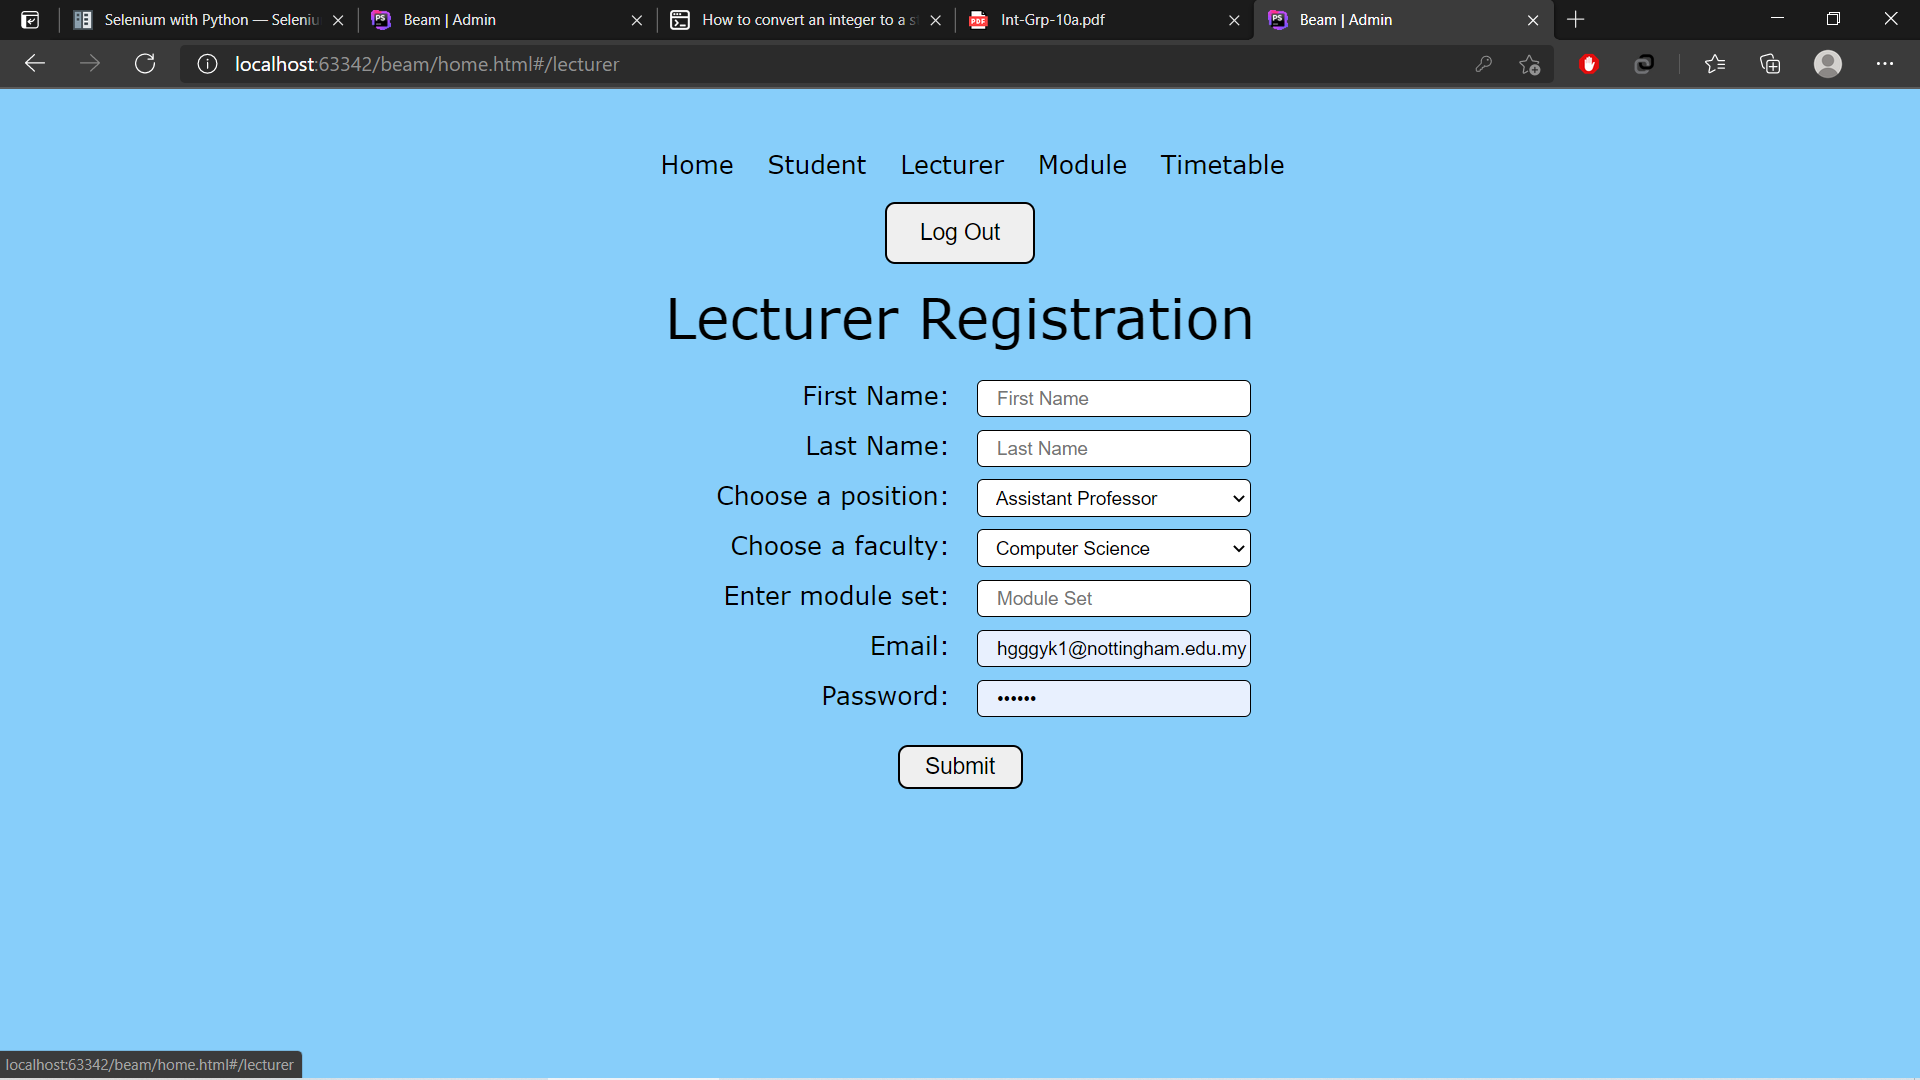
\includegraphics[width=.7\linewidth]{../images/07/01-04-lecturer-reg.png}
	\caption{This is the Lecturer Registration interface of the website}
	\label{fig:07-01-04-lecturer}
\end{figure}

\lstinputlisting[language=JavaScript,firstline=217,lastline=241]{../code/web-home.html}

When the \textit{email} and \textit{password} are sent to Firebase Authentication to create a new account for the lecturer, the \textit{first name}, \textit{last name}, \textit{position}, \textit{faculty} and \textit{email}, are entered under the \textit{lecturer} node and grouped by the lecturer account’s \textit{user uid}. Under the \textit{users} node, the role of the account (Lecturer), module set and the \textit{programme} are entered, grouped by \textit{user uid}. With the programme name, the system will fetch all the \textit{module ids} of the modules under the module \textit{set} selected and store them in the \textit{modules} node under \textit{user uid} node, which is also under \textit{users} node. The system will also register the user uid of the lecturers under \textit{lecturers} node of each \textit{modules} node.

\bigskip
\subsubsection{Module Component}
\begin{figure}[H]
	\centering
	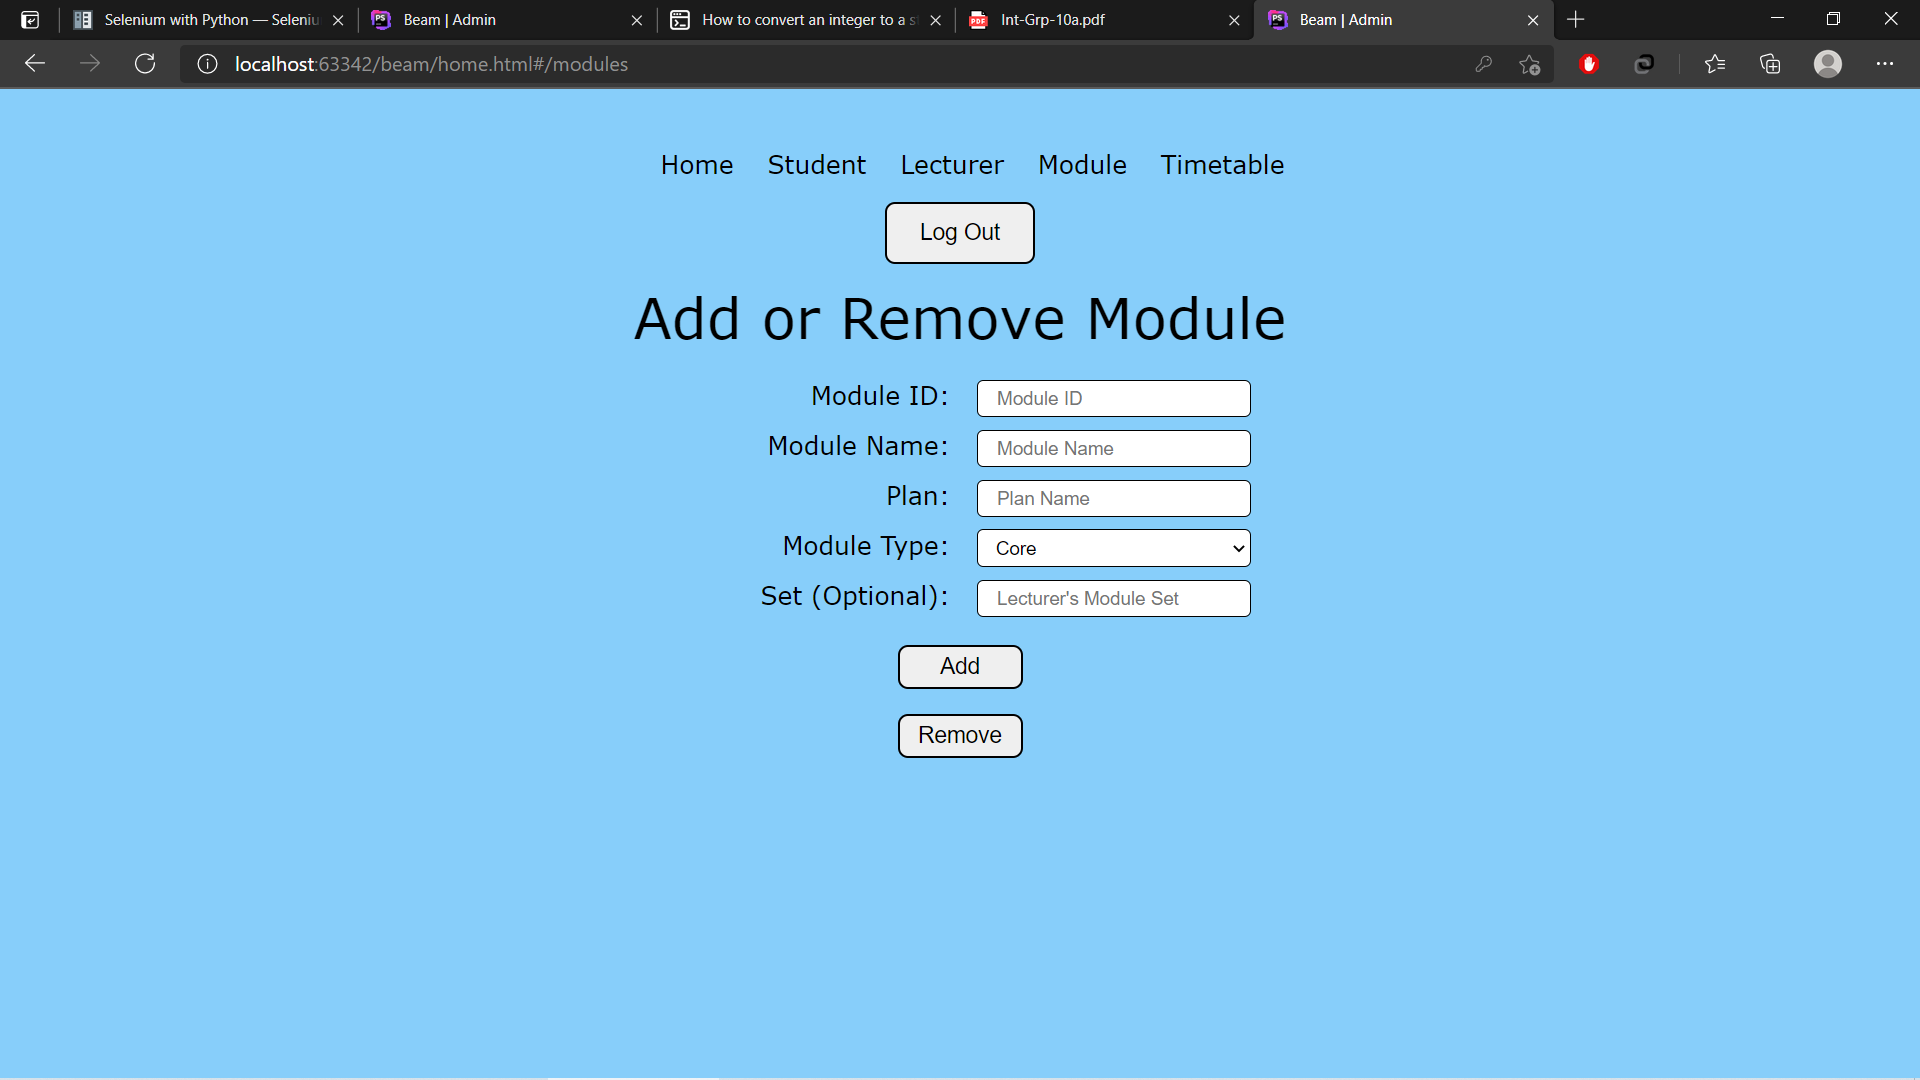
\includegraphics[width=.7\linewidth]{../images/07/01-05-module.png}
	\caption{This is the Add or Remove Module interface of the website}
	\label{fig:07-01-05-module}
\end{figure}

\lstinputlisting[language=JavaScript,firstline=276,lastline=299]{../code/web-home.html}

To add module details to the database, the system will enter the \textit{module names} under the \textit{module id}, which is under the \textit{modules} node. By the names of the \textit{academic plan} which the \textit{modules} fall under, the \textit{modules ids} of these \textit{modules}, grouped by \textit{module type}, will be placed under the \textit{plan name}, which is under the \textit{plan} node. For the modules taught by a lecturer, the \textit{module ids} will be stored under \textit{module set}, under the modules' \textit{plan name}, which is also under the \textit{plan} node.

\lstinputlisting[language=JavaScript,firstline=300,lastline=311]{../code/web-home.html}

To delete module details from the database, fetch the \textit{module id} from the website and query the modules and remove the data under the matched \textit{module id}. The system can remove the same module ids from the database directory: \textit{plan/plan name/module type}. 

\bigskip
\subsubsection{Timetable Component}
\begin{figure}[H]
	\centering
	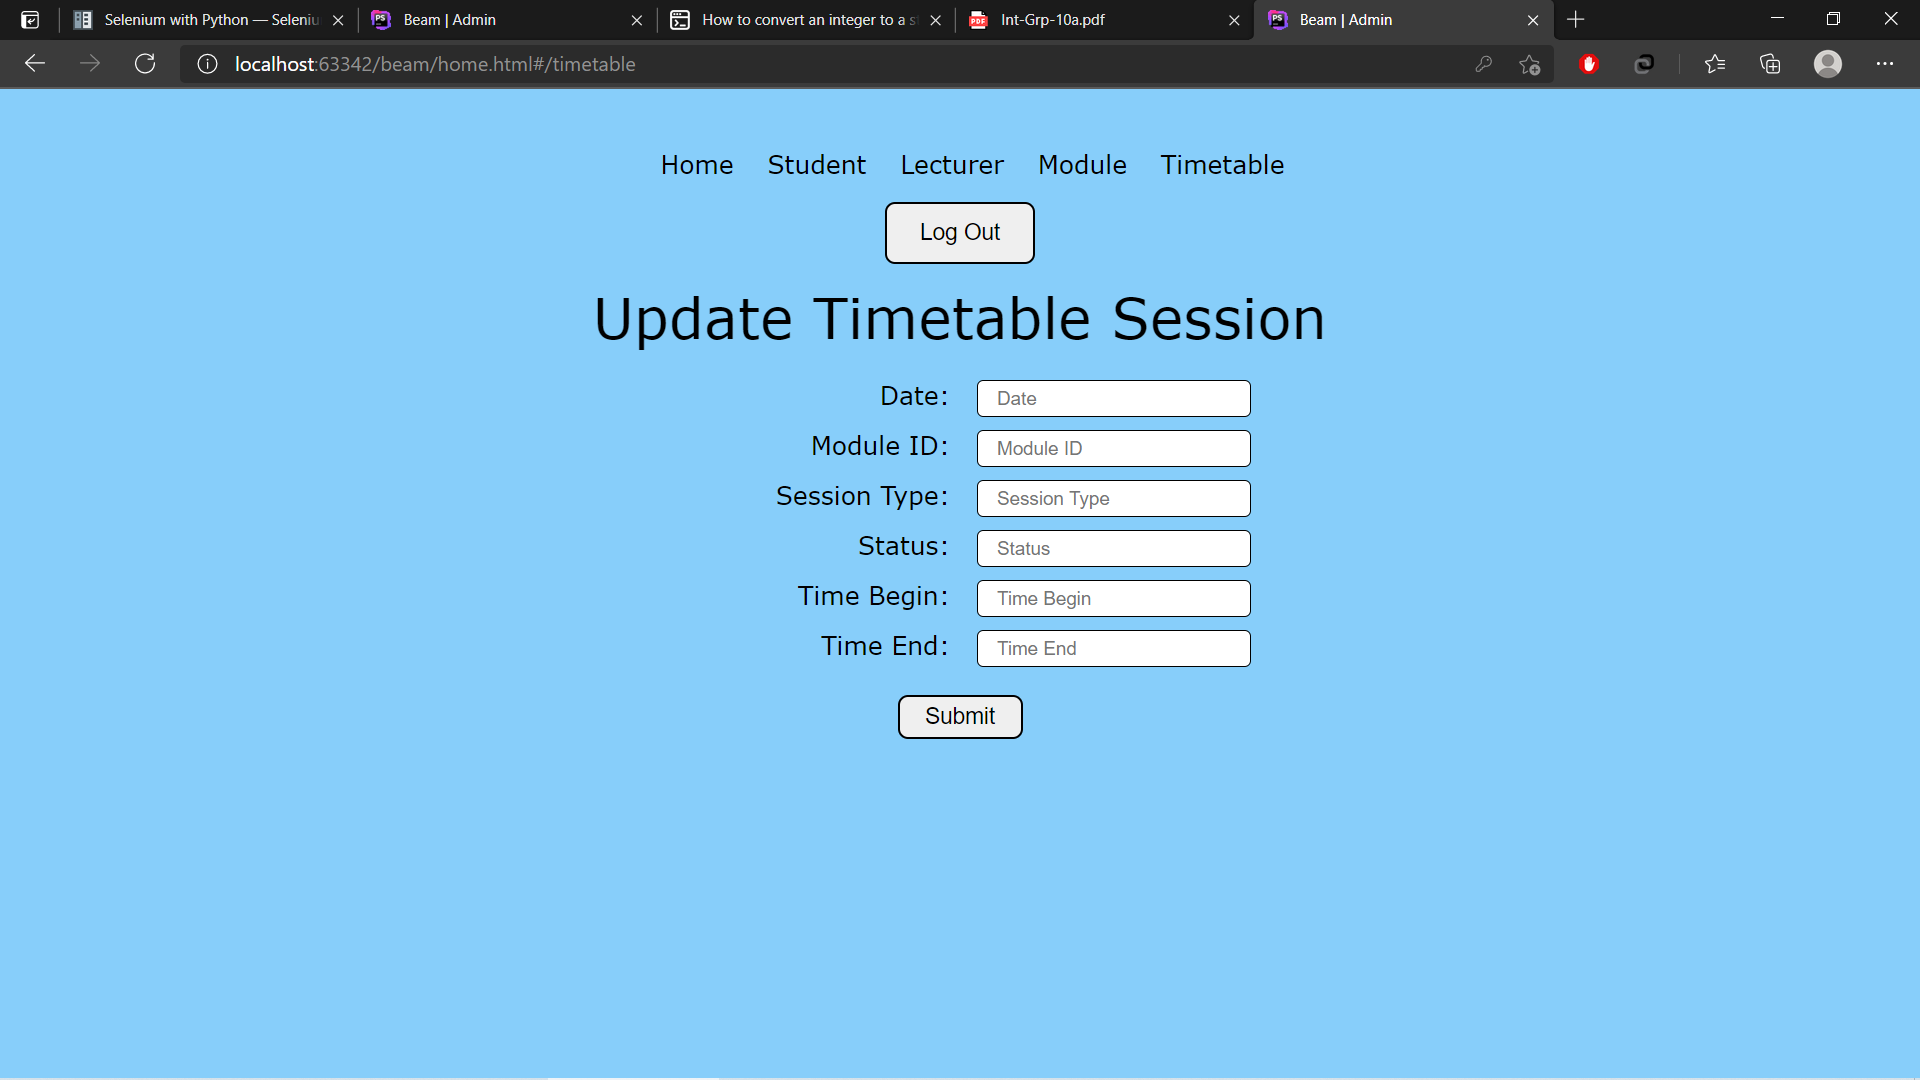
\includegraphics[width=.7\linewidth]{../images/07/01-06-timetable.png}
	\caption{This is the Update Timetable Session interface of the website}
	\label{fig:07-01-06-timetable}
\end{figure}

\lstinputlisting[language=JavaScript,firstline=334,lastline=356]{../code/web-home.html}

The system sends the \textit{date}, \textit{module\_id}, \textit{session type}, \textit{session status} (Opened/Closed), \textit{time\_begin}, and \textit{time\_end} to the database. Under the \textit{timetable} node, the module details will be entered, grouped by the \textit{date}. Under the \textit{modules\_session} node, the module details will be entered, grouped by the \textit{module\_id}. This groups the sessions of a module under a \textit{module\_id}.

\bigskip
\subsection{Test Results}
The changes reflected in the database due to the Python script will be shown below in screenshots
\begin{figure}[H]
	\centering
	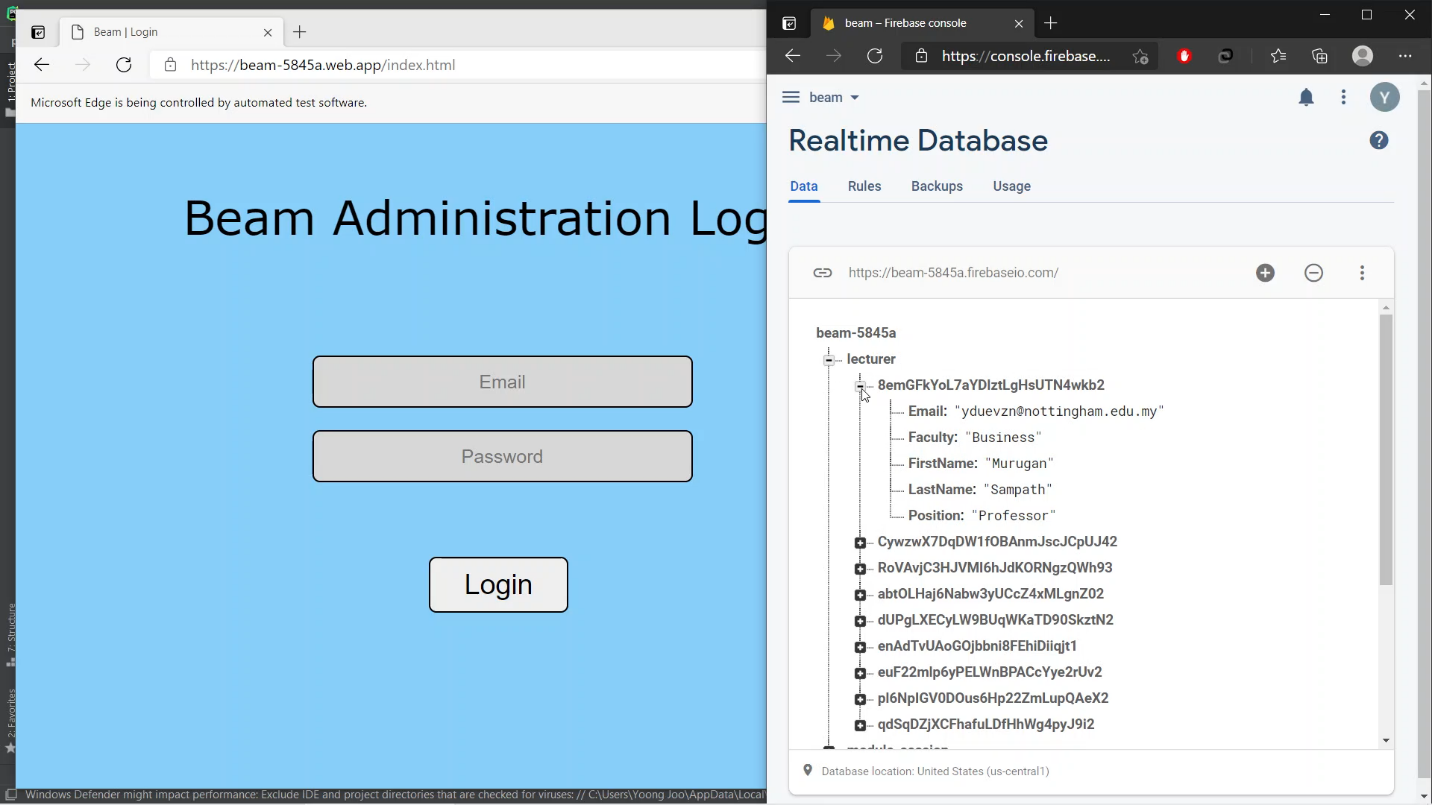
\includegraphics[width=.7\linewidth]{../images/07/01-07-test-lecturer.png}
	\caption{Changes made to the lecturer node}
	\label{fig:07-01-07-test-lecturer}
\end{figure}
\begin{figure}[H]
	\centering
	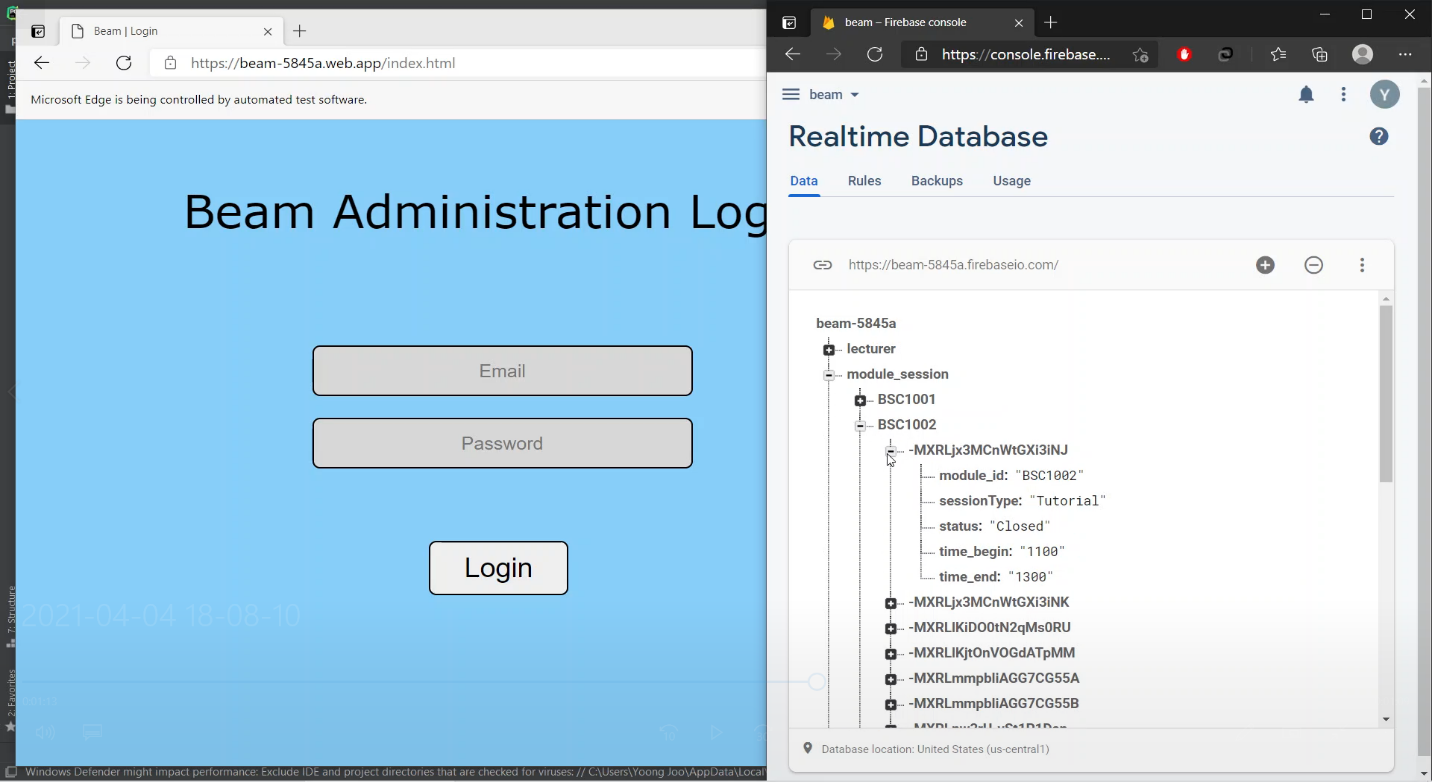
\includegraphics[width=.7\linewidth]{../images/07/01-08-test-module-session.png}
	\caption{Changes made to the module\_session node}
	\label{fig:07-01-08-test-module-session}
\end{figure}
\begin{figure}[H]
	\centering
	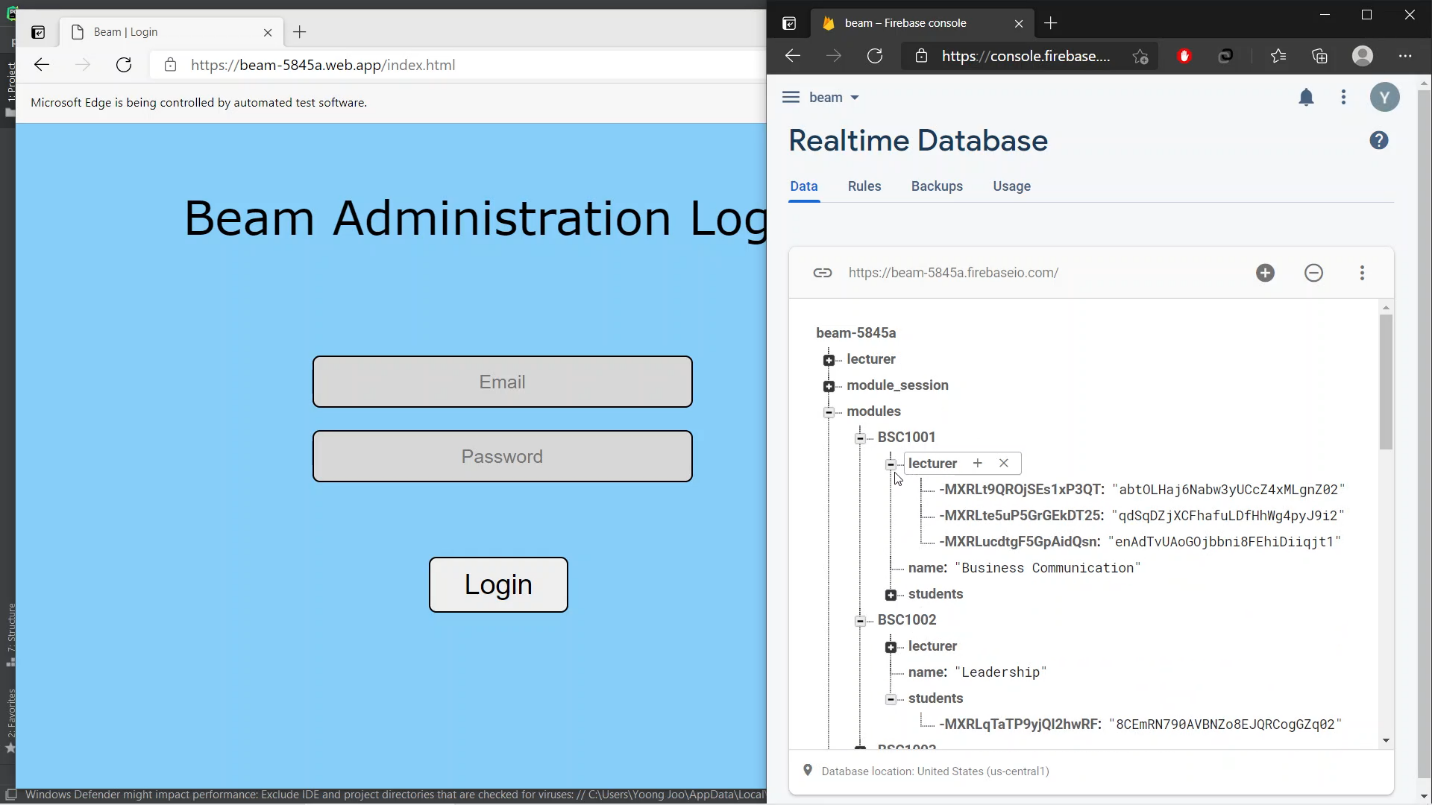
\includegraphics[width=.7\linewidth]{../images/07/01-09-test-module.png}
	\caption{Changes made to the modules node}
	\label{fig:07-01-09-test-module}
\end{figure}
\begin{figure}[H]
	\centering
	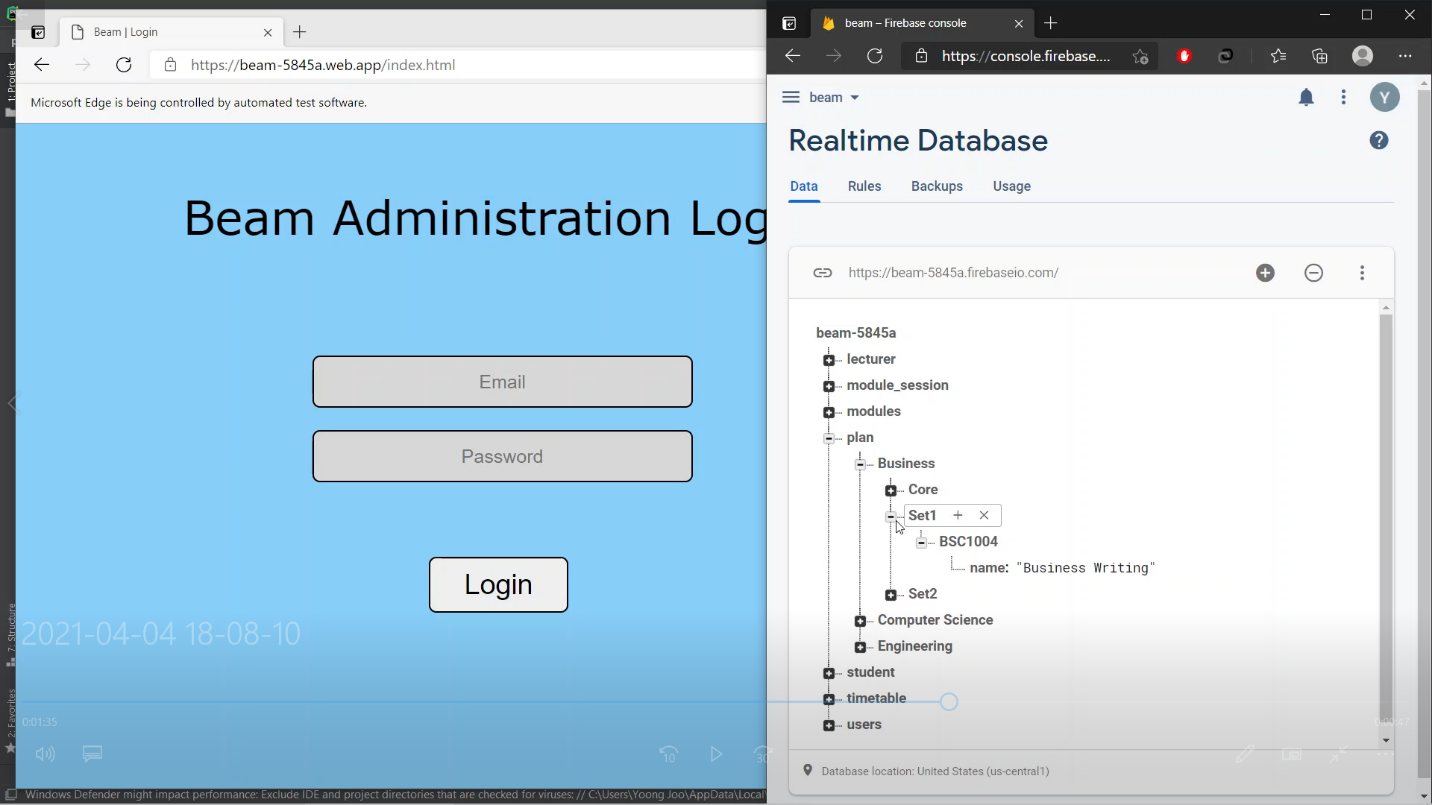
\includegraphics[width=.7\linewidth]{../images/07/01-10-test-plan.png}
	\caption{Changes made to the plan node}
	\label{fig:07-01-10-test-plan}
\end{figure}
\begin{figure}[H]
	\centering
	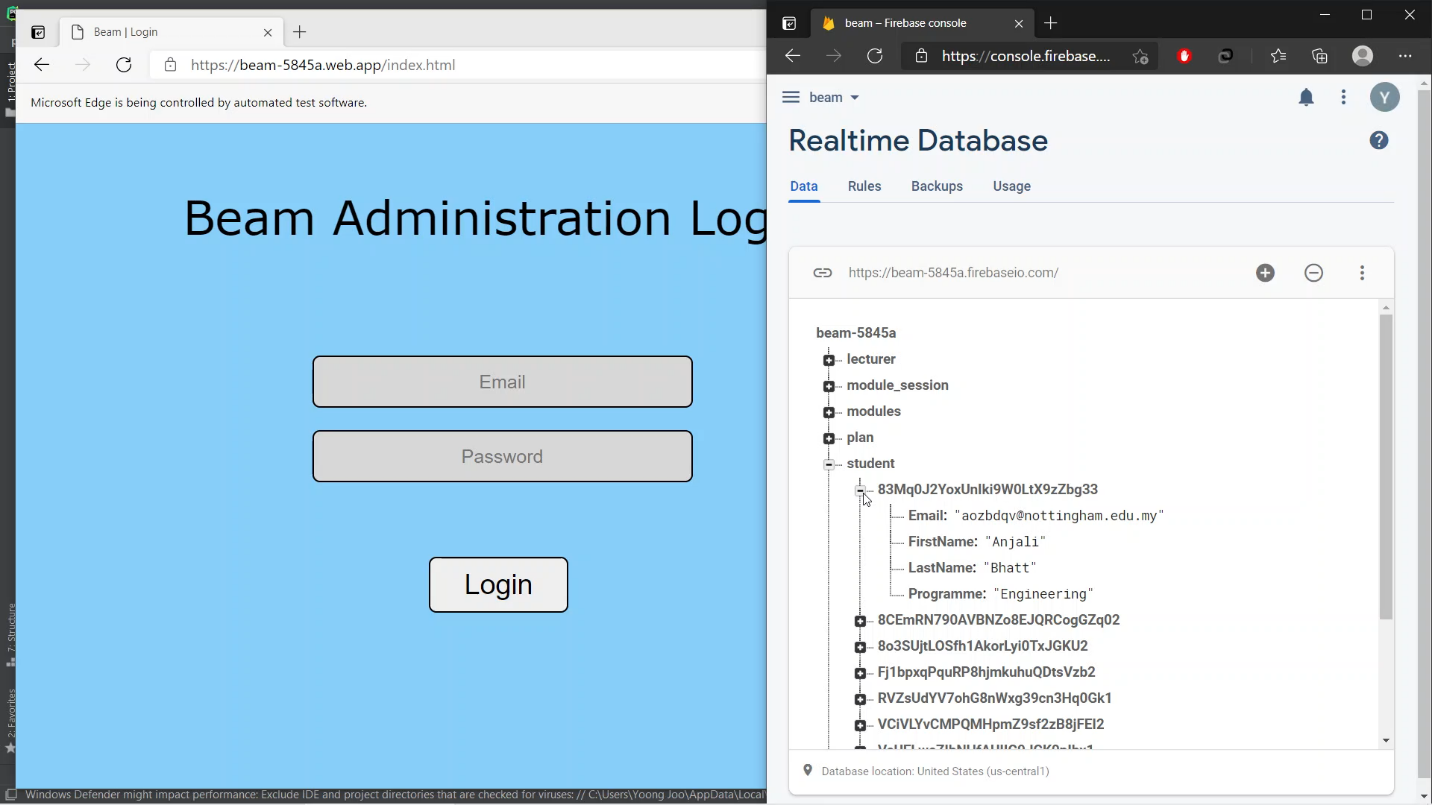
\includegraphics[width=.7\linewidth]{../images/07/01-11-test-student.png}
	\caption{Changes made to the student node}
	\label{fig:07-01-11-test-student}
\end{figure}
\begin{figure}[H]
	\centering
	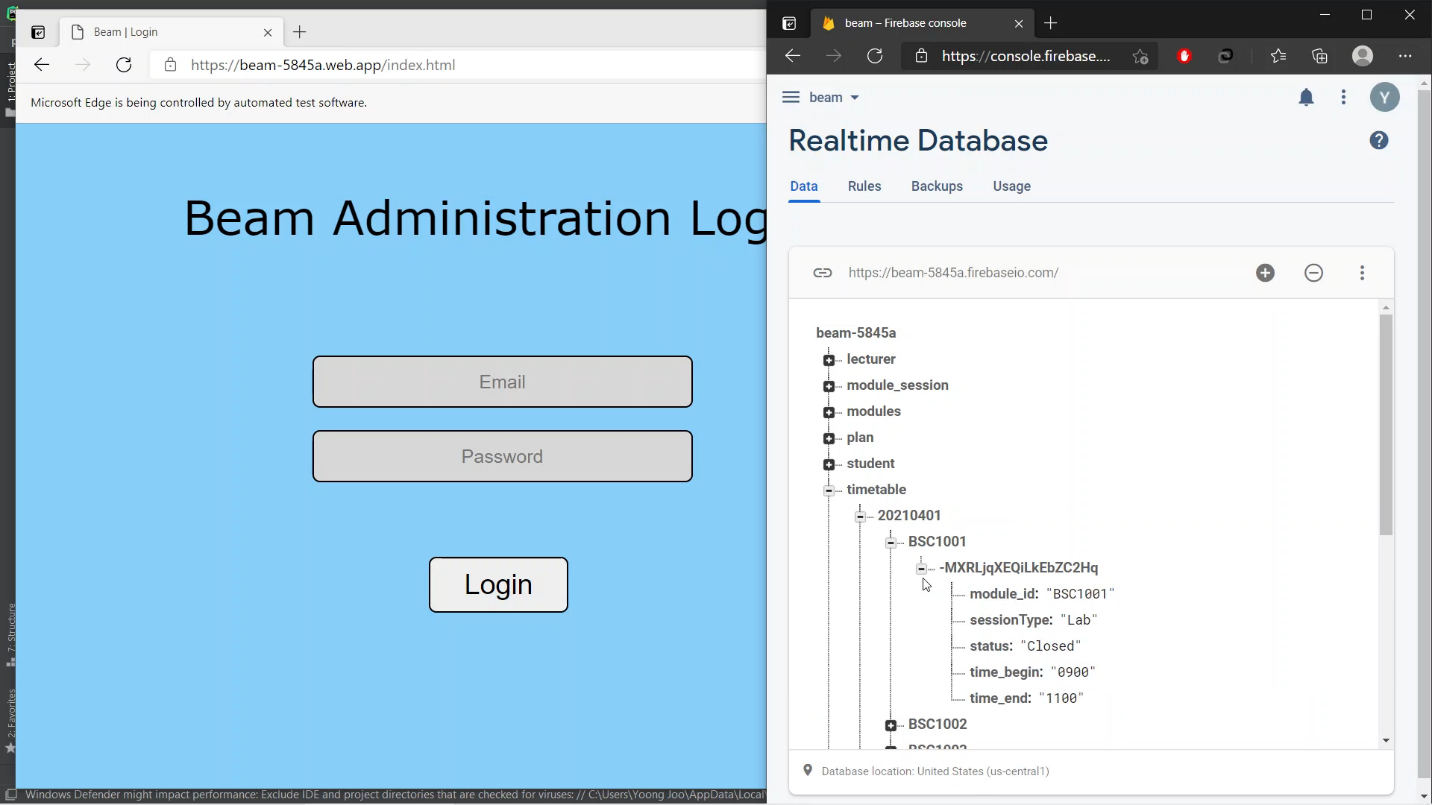
\includegraphics[width=.7\linewidth]{../images/07/01-12-test-timetable.png}
	\caption{Changes made to the timetable node}
	\label{fig:07-01-12-test-timetable}
\end{figure}
\begin{figure}[H]
	\centering
	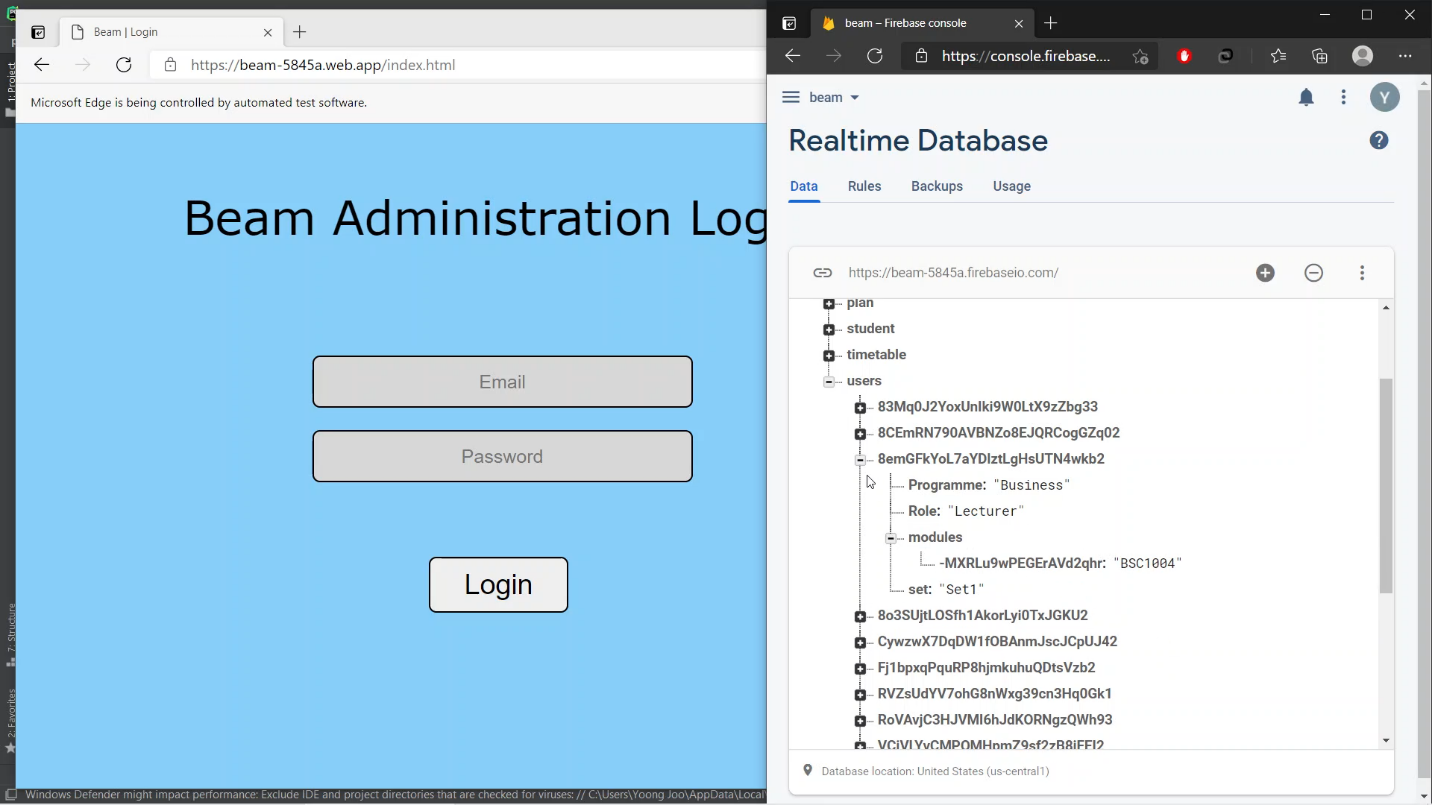
\includegraphics[width=.7\linewidth]{../images/07/01-13-test-users.png}
	\caption{Changes made to the users node}
	\label{fig:07-01-13-test-users}
\end{figure}

\section{Application}
\subsection{Overview of Classes}
\begin{figure}[H]
	\centering
	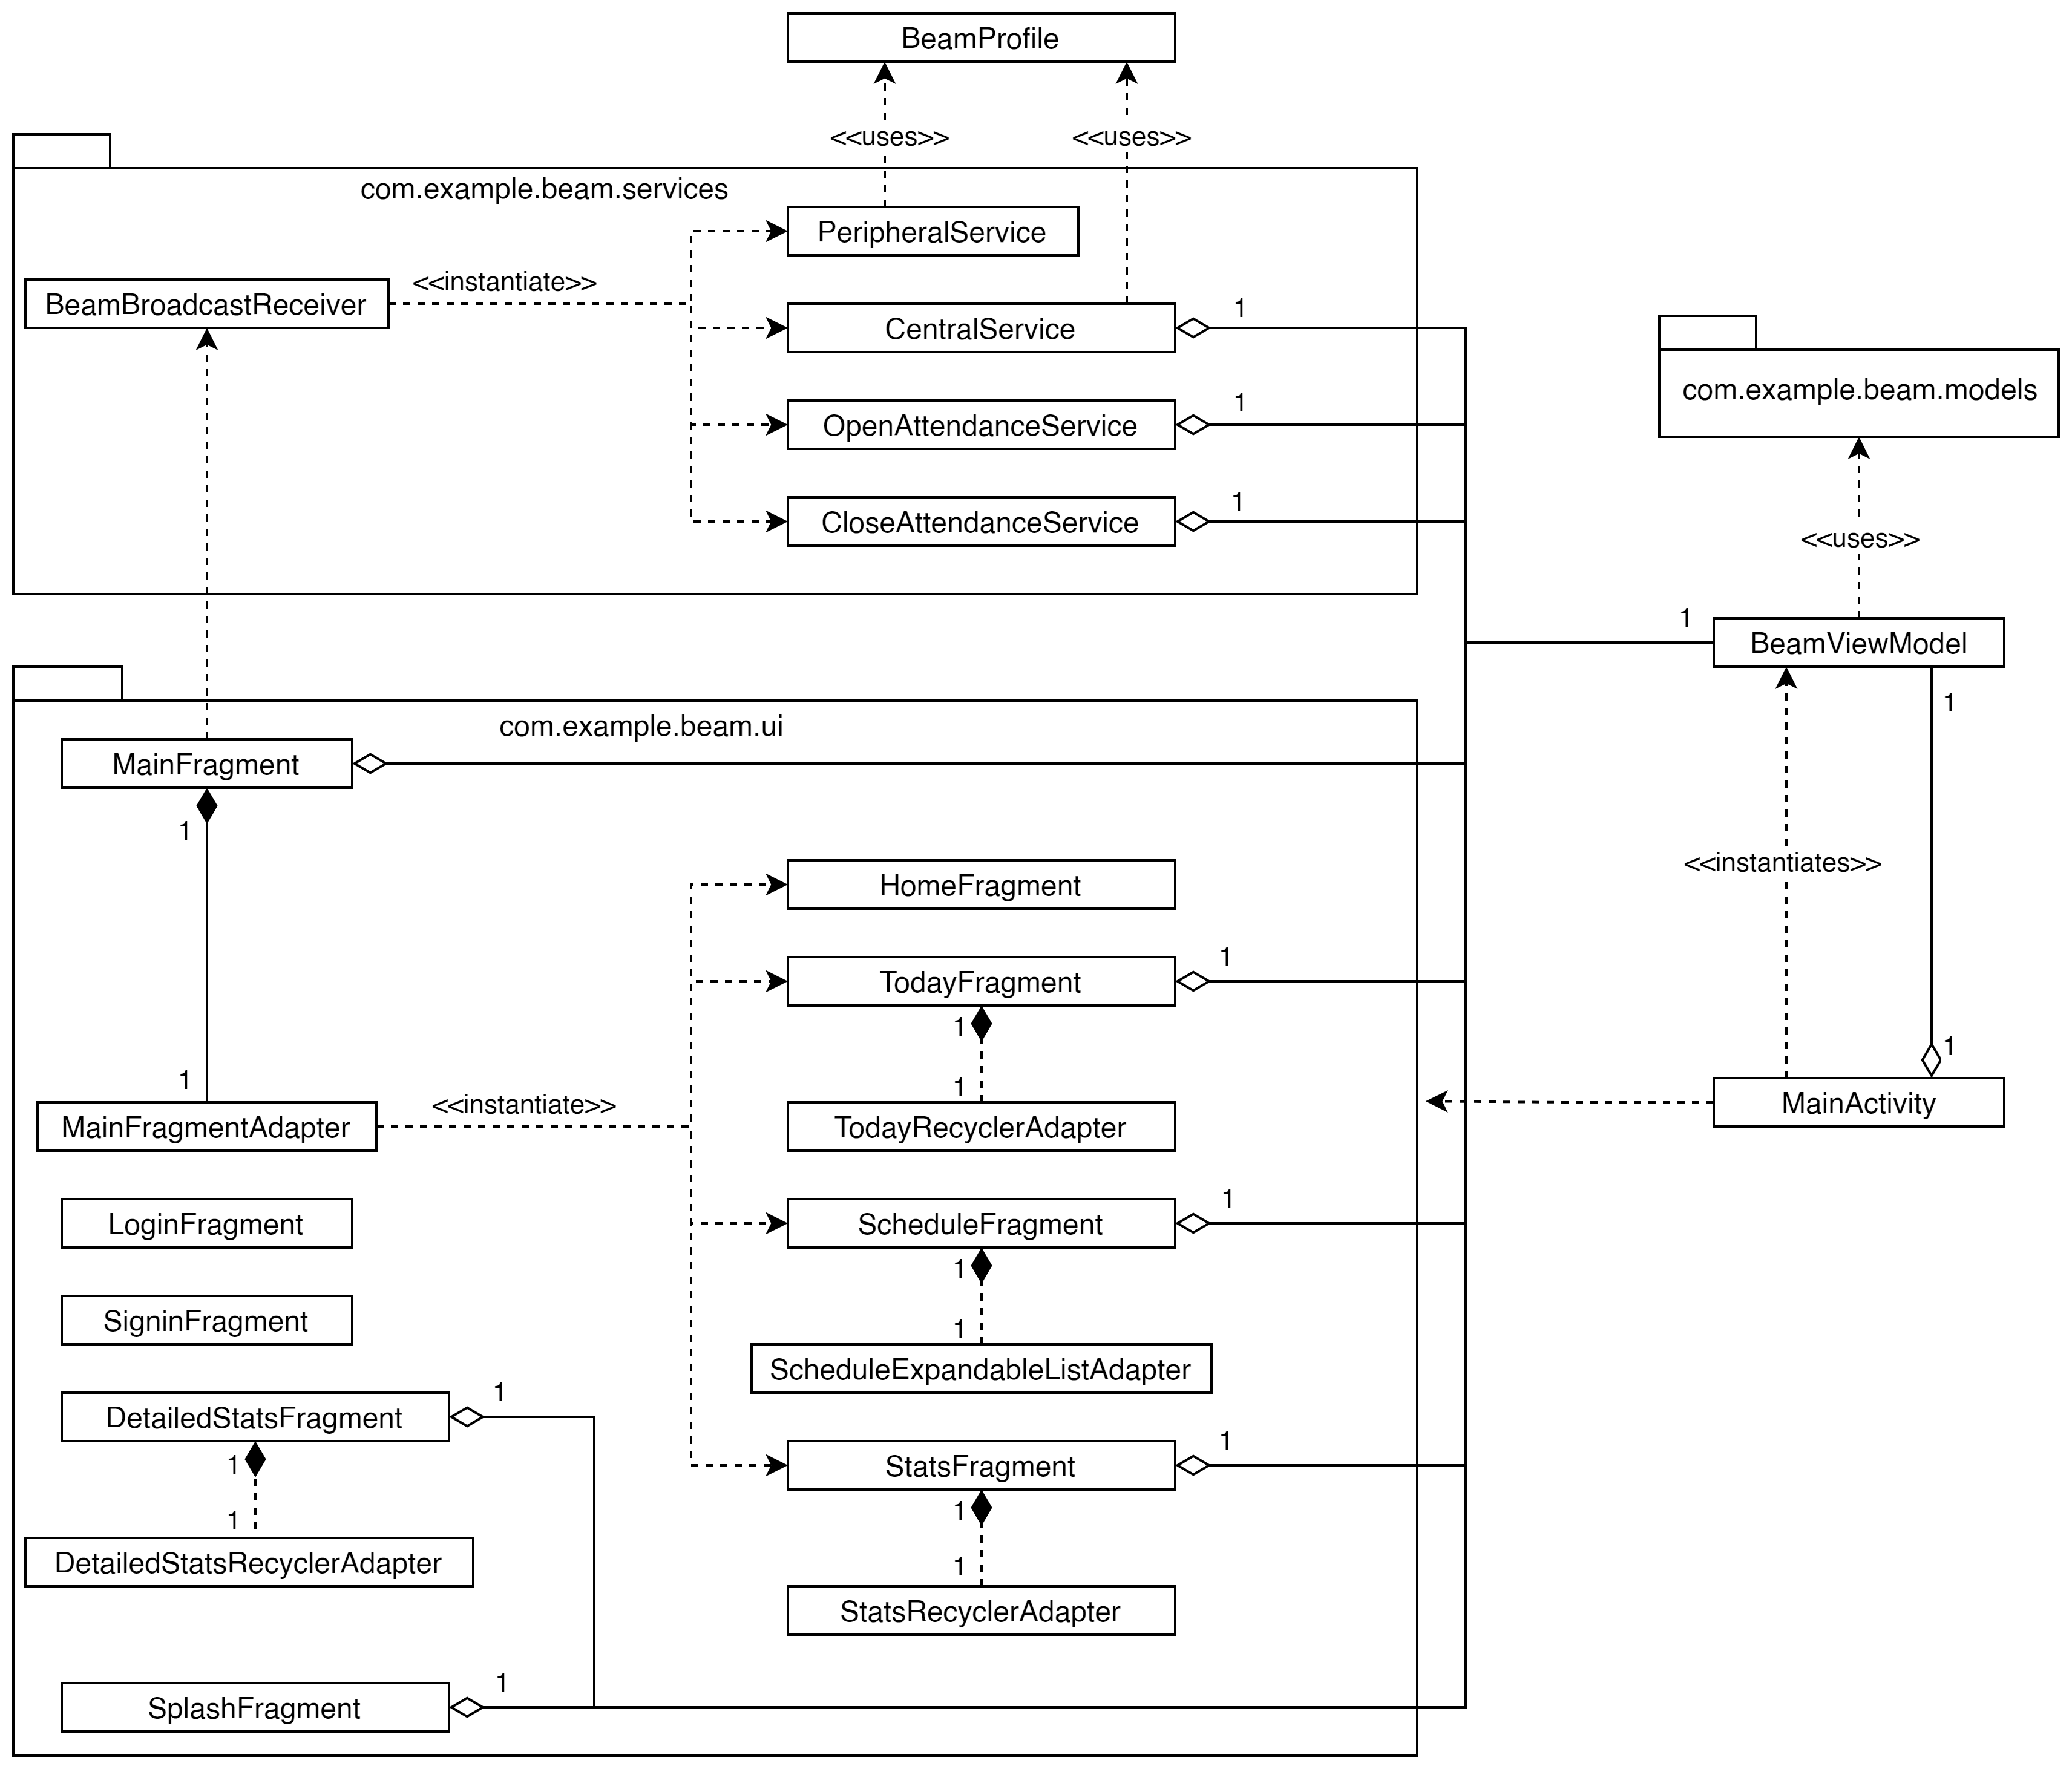
\includegraphics[width=.8\linewidth]{../images/07/02-01-class-diagram.png}
	\caption{Class diagram of custom classes}
	\label{fig:07-02-01-class-diagram}
\end{figure}
The application has many dependencies on external libraries, so the class diagram above only contains relationships between custom classes for the app. The diagram is non-exhaustive and is instead meant to convey how the classes are involved in the 3 different functions of the app: UI, fetching data from the database, and attendance taking.

The \textit{ui} package is self-explanatory in that its main purpose is for the application UI. \textit{BeamViewModel} and classes within the \textit{models} package are responsible for fetching data from the Firebase Realtime Database. Lastly, classes in the \textit{services} package along with \textit{MainFragment} and \textit{BeamProfile} are responsible for the attendance taking functionality. 

\subsection{Splash Screen}

\subsection{Login Screen}

\lstinputlisting[language=Java]{../code/app-login-function.java}

The login function gets the user input of email and password from the app and trim the input to remove whitespace from both sides of a string. It will send out an alert to the user if the user doesn’t enter email or password before submitting. If the login is successful verified by Firebase Authentication, the user will be redirected to the Home Screen. If not, the function sends an alert which state the login error. 

\bigskip
\subsection{Home Screen}
The home screen (implemented as \textit{MainFragment}) is the ``start destination" which the user arrives at first. However, if there is no authentication state or on first load of the app, the user is redirected to the splash screen. The home screen contains a \textit{ViewPager2} that consists of 4 fragments: \textit{HomeFragment}, \textit{TodayFragment}, \textit{ScheduleFragment}, and \textit{StatsFragment}. These fragments can be accessed by swiping on the screen. \textit{HomeFragment} just contains a rippling animation and no functionality. 

\textit{TodayFragment} utilises a \textit{RecyclerView} to display the sessions of the day in a list. The data is fetched using an instance of \textit{BeamViewModel} and the list of sessions is passed to the \textit{TodayRecyclerAdapter} to populate the \textit{RecyclerView}. \textit{TodayRecyclerAdapter} inflates a layout for each row of the list and creates as many rows as needed.

\textit{ScheduleFragment} utilises an \textit{ExpandableListView} to display a multi-level list. The first level consists of 7 rows, one for each day of the week. Each row can be expanded into a second level that displays the sessions of the particular day. Data is fetched using an instance of \textit{BeamViewModel} and the weekly timetable is passed to \textit{ScheduleExpandableListAdapter} which is responsible for inflating a layout for each row of the multi-level list.

\textit{StatsFragment} utilises a \textit{RecyclerView} to display the attendance statistics of each module. Data of the student’s attendance history is fetched via an instance of \textit{BeamViewModel} and is passed to an instance of \textit{StatsRecylerAdapter}. \textit{StatsRecyclerAdapter} inflates layouts for each row and calculates the attendance percentage for each module.

\subsection{Settings Screen}

\lstinputlisting[language=Java]{../code/app-settings-screen.java}

The settings screen (implemented by \textit{SettingsFragment}) contains a single button for logging out. When pressed, the user’s authentication state is deleted, and the user is redirected to the home screen. Due to lack of authentication state, the user is again redirected to the login screen.

\bigskip
\subsection{Data Fetching Classes}
The application has integrated google firebase within its code with specified ID, connecting it to the database. When the app first started, it will initialize its connection with the database, which is needed to send and receive data. The classes responsible for fetching data are those within the \textit{models} package and the \textit{BeamViewModel} class. The classes within \textit{models} package are used to store data fetched from the database. When there is data to be collected, the app will request from the database, then it will create new objects (instances of classes in \textit{models} package) to store the data. The main fetching of data is handled by \textit{BeamViewModel}.

\textit{BeamViewModel} extends Android’s \textit{ViewModel} and contains several \textit{MutalbleLiveData} instances from which other classes (within the app) may observe changes in. Instances of \textit{BeamViewModel} are unique to each Android \textit{Activity}. The data stored includes user details, weekly timetable, attendance history, and enrolled modules. The class uses Firebase’s \textit{ValueEventListeners} to ``listen" to changes in certain parts of the database. 

\subsection{BLE Services and Related Classes}
The main attendance taking functionality is mainly handled by the classes declared in the services package except for \textit{MainFragment} and \textit{BeamProfile}.

\textit{BeamProfile} describes the custom GATT profile which the app uses. The profile is exactly as described in \hyperref[sec:gatt-profile]{Section 5.1}. The class defines constants for UUIDs of the service, characteristics, and descriptors.

\textit{MainFragment} in the \textit{ui} package is responsible for scheduling alarms for each session during the day. On arrival at the \textit{MainFragment}, the class schedules alarms (for upcoming sessions in the day) to broadcast the start of the BLE services. The broadcasts contain an Android \textit{Intent} with extras (additional data) of request codes (of which service to start/stop), module ID, and session ID of the session taking place. The \textit{BeamBroadcastReceiver} class receives the broadcasts (at the start of a session) and depending on the request codes, either begins a service for taking attendance or opening attendance. An \textit{Intent} is passed to these services containing the extras of module ID and session ID. This is used as the attendance token (a concatenation of module ID and session ID).

There are 4 services declared for this app. The first is \textit{CentralService} which is the service responsible for taking a student’s attendance. The \textit{CentralService} periodically scans for BLE devices that are advertising the \textit{BeamProfile}. Once it detects a device, it stops scanning and attempts to connect with the device. It reads the attendance token from the device and compares with one it formed from the \textit{Intent}. If it is a match, the service updates the attendance records in the database, notifies the user that attendance is taken, and starts the \textit{PeripheralService}.

The \textit{PeripheralService} is responsible for advertising the \textit{BeamProfile} and allowing other devices to read the attendance token. The service ``sends out" the attendance tokens for a certain time period. If no connections were made to any devices within that time period, the service automatically stops. If a connection is made, the service will refresh the timer for stopping the service.

The \textit{OpenAttendanceService} is started only by lecturers' devices and responsible for updating attendance records in the database. For the session, the service initially sets the attendance for each student in the module as false. The service also updates the status of the session to ``Open" in the database. The service then starts the \textit{PeripheralService} and passes the module ID and service ID through an \textit{Intent}. The \textit{CloseAttendanceService} updates the status of the session to ``Closed" in the database. This is scheduled to run at the end of a session.

\subsection{Test Results}
Regarding application UI, all tests in the UI test suite passed. Swiping between screens, pressing buttons, and back navigation worked as intended. 

Regarding attendance taking functionality, most of the tests passed. The starting of scheduled background services at specific time windows functioned as intended. The test for advertising of the attendance by the initial peripheral device passed. Tests for initial and subsequent scans for BLE capable devices by the central device passed. BLE connection between peripheral and central devices along with writing attendance to the database functioned as intended. The only test to fail is the switching from central role to a peripheral role in the initial central device. After receiving the attendance token, the central device (now switching to a peripheral role) failed to start advertising the Beam Service UUID. This test failed on one device and passed on another device. However, the test did not consistently fail. A possible explanation is variations between Bluetooth components of the two devices. This is only speculation and has not been confirmed.  

\end{document}